\documentclass[10pt,a4paper,twoside]{report}

%LOAD PACKAGES
\usepackage[T1]{fontenc}
\usepackage[italian,english]{babel}
\usepackage{hyperref}
\addto\extrasenglish{%
	\def\chapterautorefname{Chapter}}
\addto\extrasenglish{%
	\def\subsectionautorefname{section}}
\usepackage{graphicx}
\usepackage{rotating}
\usepackage{tabularx}
\usepackage{amsmath}
\usepackage{listings}
\usepackage[printonlyused,withpage]{acronym}
\usepackage{frontespizio}
\usepackage{imakeidx}
\usepackage{comment}
\usepackage[table,usenames,dvipsnames]{xcolor}
\usepackage{xcolor}
\usepackage{setspace}
\usepackage{titlesec}
\usepackage{chemformula}
\usepackage{varioref}
\usepackage{subfigure}
\usepackage{alphalph}
\usepackage{siunitx}
\usepackage{multirow}
\usepackage{array}
\usepackage[nottoc]{tocbibind}
\usepackage[a4paper]{geometry}
\usepackage{pdfpages}


%\usepackage{url}
%\usepackage{listings}
%\usepackage[toc]{appendix}

%[display]

\titleformat{\chapter}%
  {\normalfont\bfseries\huge}{\thechapter.}{10pt}{}

% Cartelle da cui recuperare le immagini
\graphicspath{{immagini/}, {grafici/}, {first/}, {second/}, {third/},{fourth/}, {fifth/}}

%Indice
%\makeindex

%Indice dei contenuti
\hypersetup{
    colorlinks = false,
    allbordercolors = {white}
}

%Numerazione subsubsection
\setcounter{tocdepth}{3}
\setcounter{secnumdepth}{3}


%COMMAND TO INCREASE POSSIBLE LABELS IN CAPTION
\renewcommand*{\thesubfigure}{(\alphalph{\value{subfigure}})}

%COMMAND TO DEFINE NEW TYPE OF COLUMN(per andare a capo e centrare il testo)
\newcolumntype{C}[1]{>{\centering\let\newline\\\arraybackslash\hspace{0pt}}m{#1}}

%VARIOREF
\vrefwarning






%------------------------------------
%		INFO
%------------------------------------

%\title{Studio di rivelatori a pixel monolitici CMOS per l'upgrade dell'esperimento Belle II}
%\author{Mara Stefania Calò}
%\date{9 Novembre 2022}
%\newcommand{\institution}{Università di Pisa}
%\newcommand{\department}{Dipartimento di Fisica}

%--------------------------------------
%		TITLE
%--------------------------------------


\begin{document}

%Contenuti
\doublespacing
\tableofcontents
\singlespacing


\begin{comment}
\begin{frontespizio}
\Universita{Pisa}
\Logo[scale=.1]{logo}
\Dipartimento{Fisica}
\Corso{Fisica delle Interazioni Fondamentali}
\Titolo{Studio di rivelatori a pixel monolitici CMOS per l'upgrade dell'esperimento Belle II}
\Candidato{Mara Stefania Calo'}
\Relatore{prof. Francesco Forti}
\Annoaccademico{2022.2023}
\end{frontespizio}
\end{comment}

\newpage

% --------------------------------------------
%		ABSTRACT 
%---------------------------------------------
\section*{Abstract}

\begin{comment}
Belle II è un esperimento di fisica delle particelle situato a Tsukuba, in Giappone, nel laboratorio (di) KEK (100 km da Tokyo). E' una flavor-factory di seconda generazione che opera alla frontiera dell'intensità, detenendo il record mondiale di maggiore luminosità. L'acceleratore SuperKEKB è un collider di fasci $e^{+}$ $e^{-}$ con energie asimmetriche e piccate alla risonanza $\Upsilon$(4S). Auspica a raccogliere un set di dati fino a 50 $ab^{-1}$ (x50 Belle dataset, x100 BaBar dataset) per studiare la violazione di CP nei mesoni B e ricerca nuova fisica oltre il Modello Standard.
\end{comment}


% --------------------------------------------
%		CAPITOLO 1 
%---------------------------------------------

\input{first\_chapter}



% --------------------------------------------
%		CAPITOLO 2 
%---------------------------------------------
\chapter{Upgrade di Belle II}
%\addcontentsline{toc}{chapter}{Upgrade di Belle II}

%---------------------------------------------
%			2.1
%---------------------------------------------
\section{Sorgenti di background e limitazioni di Belle II}
%\addcontentsline{toc}{section}{Sorgenti di background e limitazioni di Belle II}

\subsection{Effetto Touschek}

\subsection{Beam-gas scattering}

\subsection{Radiative Bhabha scattering e processi a due fotoni}

\subsection{Radiazione di sincrotrone (SR)}

\subsection{Instabilità ''Head-tail''}

\subsection{Stato attuale del background e implicazioni future}


%---------------------------------------------
%			2.2
%---------------------------------------------
\section{Motivazioni per l'upgrade}
%\addcontentsline{toc}{section}{Motivazioni per l'upgrade}

%% Incremento del background per raggiungere elevate luminosità
%% Degradazione dei componenti del rivelatore
%% Occupancy e radiation hardness
%% Riduzione del materiale interposto (dei rivelatori) per permettere maggiore risoluzione a bassi impulsi



%---------------------------------------------
%			2.3
%---------------------------------------------
\section{Sommario di possibili upgrade}
%\addcontentsline{toc}{section}{Sommario di possibili upgrade}

\subsection{DEPFET}

\subsection{Thin sensor}

\subsection{CMOS MAPS}

\subsection{SOI}


% --------------------------------------------
%		CAPITOLO 3 
%---------------------------------------------
\chapter{Il rivelatore VTX}
%\addcontentsline{toc}{chapter}{Il rivelatore VTX}


%---------------------------------------------
%			3.1
%---------------------------------------------
\section{Layout del rivelatore VTX}
%\addcontentsline{toc}{section}{Layout del rivelatore VTX}

\subsection{iVTX}

\subsection{oVTX}


%---------------------------------------------
%			3.2
%---------------------------------------------
\section{Simulazioni di performance}
%\addcontentsline{toc}{section}{Simulazioni di performance}


%---------------------------------------------
%			3.3
%---------------------------------------------
\section{Caratteristiche chip sensore}
%\addcontentsline{toc}{section}{Caratteristiche chip sensore}

%% OBELIX


%---------------------------------------------
%			3.4
%---------------------------------------------
\section{Struttura meccanica}
%\addcontentsline{toc}{section}{Struttura meccanica}

%% Struttura Layer
%% Sistema di cooling 
%% Connessioni?


% --------------------------------------------
%		CAPITOLO 4
%---------------------------------------------
\chapter{Sensori CMOS MAPS}
%\addcontentsline{toc}{chapter}{Sensori CMOS MAPS}


\section{Rivelatori a semiconduttore}
%\addcontentsline{toc}{section}{Rivelatori a semiconduttore}

\section{Sensori a pixel monolitici/ibridi}
%\addcontentsline{toc}{section}{Sensori a pixel monolitici/ibridi}

\section{Tecnologia CMOS MAPS}
%\addcontentsline{toc}{section}{Tecnologia CMOS MAPS}

\begin{comment}
small fill factor /large fill factor
\end{comment}

\section{Storia degli sviluppi di Monopix}
%\addcontentsline{toc}{section}{Storia degli sviluppi di Monopix}



% --------------------------------------------
%		CAPITOLO 5
%---------------------------------------------

\chapter{Caratterizzazione di TJ-Monopix 2}
%\addcontentsline{toc}{chapter}{Caratterizzazione di TJ-Monopix 2}

\section{Matrice e flavor}

\subsection{Funzionamento della maschera per i pixel rumorosi}

\subsection{Readout analogico e digitale}

\subsubsection{Reset del BCID}
\begin{comment}
REFERENZE
\end{comment}

\subsubsection{Registri principali (e conversioni?)}

\subsection{Confronto degli andamenti con le simulazioni}
%\addcontentsline{toc}{subsection}{Confronto degli andamenti con le simulazioni}


\section{Caratterizzazione tramite l'iniezione}
%\addcontentsline{toc}{section}{Caratterizzazione tramite l'iniezione}

\begin{comment}
Nel prototipo sotto studio, il chip W14R12, si sono rilevate fin da subito alcune problematiche legate ai pixel della matrice, sia per quel che riguarda la parte analogica che quella digitale.
In particolare, a differenza del suo predecessore TJ-Monopix1, TJ-Monopix2 è equipaggiato da un circuito che permette il \textit{tuning della threshold}, ossia di correggere, anche se di pochi DAC, la threshold di ciascun pixel, in modo da avere una threshold globale più uniforme possibile, o comunque con una dispersione piccola quanto possibile.

Preliminarmente però, è necessario studiare la distribuzione della threshold su tutta la matrice e noi abbiamo analizzato separatamente i 4 flavor, per poter anche studiare le loro principali differenze di funzionamento e performance.

Il fine ultimo di questa misura, è anche quello di riuscire a caratterizzare il comportamento di ciascun pixel, ad una carica iniettata equivalente all'energia tipica rilasciata dagli elettroni emessi dal decadimento di materiali radioattivi, e in particolare quelli dovuti alla cattura elettronica nel \ch{^55Fe}, le cui linee di emissione sono abbastanza piccate da permettere poi di confrontare i dati più facilmente. Come spiegato meglio nel paragrafo (?????), il \ch{^55Fe} ha una prima linea di emissione a  5.9 KeV che corrisponde in media all'incirca a 1616 $e^{-}$ generati (nel pixel?). Per questa ragione, nelle misure di iniezione è necessario, in base ai valori di conversione tra DAC ed $e^{-}$ SCRIVI, arrivare ad iniettare cariche in modo da studiare il comportamento dei pixel in queste regioni maggiormente interessanti. 
\end{comment}

%------------------------------------------------------------
\subsection{Problema nel circuito di iniezione}

\begin{comment}
Nel portare avanti le misure suddette, ci si è accorti di un problema nel circuito di iniezione che ne limita il range di funzionamento: l'altezza dell'impulso di iniezione infatti, cresce linearmente come aspettato fino ad un valore di $\approx$ 140 DAC, ma al al di sopra di questo valore, il circuito non solo aumenta di poco l'altezza del segnale, ma aumenta artificialmente anche il valore della threshold di un certo $\Delta V$ (o equivalentemente $\Delta Q$, collegati dal fattore di conversione in....).
Inoltre, per altezze dell'impulso di iniezione superiori a 200 DAC, solo il valore della threshold viene aumentato, senza però incrementare in alcun modo l'effettiva carica iniettata.

Per questa problematica, la caratterizzazione della threshold e della sua dispersione su tutti i flavor della matrice, ha richiesto una serie di misure ulteriori.
\end{comment}

%-------------------------------------------------------
\subsection{Misura dello shift medio sul valore di threshold per cariche iniettate superiori a 140 DAC}

\begin{comment}
Per poter valutare dunque questo shift artificiale sul valore della threshold, per ogni flavor della matrice abbiamo effettuato due misure della threshold e sua dispersione separate:

\begin{itemize}
\item per carica iniettata pari a 140 DAC $\rightarrow$ prima della regione di saturazione;
\item per carica iniettata pari a 200 DAC $\rightarrow$ limite massimo della ragione di saturazione (da questo valore in poi, aumenta solo la threshold, non la carica effettivamente iniettata).
\end{itemize}

Per ognuna di queste misure, è stata fittata la distribuzione della threshold per poter ottenere un valore medio sull'intero flavor, e chiamando $\Q_{th, 140}$ e $\Q_{th, 200}$  rispettivamente i valori di threshold ottenuti per iniezione a 140 e 200 DAC, è stato stimato lo shift medio come:

\begin{equation}
\Delta Q = Q_{th,200} - Q_{th,140}
\end{equation}

Infine, ai dati ottenuti per impulsi di iniezioni di 200 DAC, è stato sottratto questo valore di carica, per poter estrapolare fino a un valore di 170 DAC effettivo, il comportamento dei pixel iniettati.

Si riporta nelle sezioni successive quanto ottenuto per ciascun flavor della matrice, con il metodo utilizzato per poter stimare la threshold.

\end{comment}

%--------------------------------------------------------------------
\subsection{Curva S e threshold}
%\addcontentsline{toc}{subsection}{Curva S e threshold}

\begin{comment}
Per poter ottenere il valore della threshold per ogni pixel, ciascuno di essi deve essere iniettato un numero arbitrario di volte (noi abbiamo scelto 100), per ogni valore di impulso di iniezione compreso tra un valore minimo, scelto settando il registro del chip ''\textbf{VL}'' e un valore massimo, per mezzo del registro ''\textbf{VH}'', con step a scelta da noi settato a 1.
Fissato il valore dell'impulso di iniezione, si considera la media dei 100 output ottenuti. Così facendo, per ogni pixel, si ottiene la tipica curva nota come ''\textit{S-curve}'', che matematicamente è una error function (?) e da cui si stima il valore della threshold, prendendo il valore di carica iniettata per la quale la curva è a metà della sua altezza massima. Plottando il numero di hit rilevate su ciascun pixel diviso il numero totale, per ogni valore di carica iniettata, la metà altezza corrisponde al valore di carica per la quale il pixel rileva 50 hit su 100 totali iniettate e cioè ha un'occupancy di 0.50.

SPIEGARE METODO DI LUDOVICO????

METTI FIGURA
\begin{figure}
\centering
\includegraphics[]{}
\caption{Esempio di S-curve e stima della threshold}
\label{ex_scurve}
\end{figure}

\end{comment}

\subsubsection{Normal FE}

\begin{comment}

Come spiegato in sezione (.........METTI) il primo flavor della matrice è il \textbf{Normal}, che comprende 512 righe (0-511) e 224 colonne (0-223) per un totale di 114.688 pixel.
In figura (...) sono plottate tutte le s-curve dei pixel del primo flavor. I registri del chip sono stati settati con gli stessi valori utilizzati durante il Test Beam a Desy che sono riportati in seguito:

COLORAAAAAAAA

\begin{table}
\centering
\begin{tabular}{c|c}
Registri & Default Settings (''GOE'') \\
\hline
ITHR & 64 \\
\hline
IBIAS & 50 \\
\hline
VRESET & 143 \\
\hline
ICASN & 0 \\
\hline
VCASP & 93 \\
\hline
VCASC & 228 \\
\hline
IDB & 100 \\
\hline
ITUNE & 53 \\
\hline
VCLIP & 255 \\
\hline
ICOMP & 80 \\
\hline
IDEL & 88 \\
\hline
IRAM & 50 \\
\hline
\end{tabular}
\caption{Settings dei principali registri utilizzati per il chip W14R12, flavors Normal e Cascode, durante il Test Beam a Desy.}
\label{tb_settings}
\end{table}

\begin{figure}
\centering
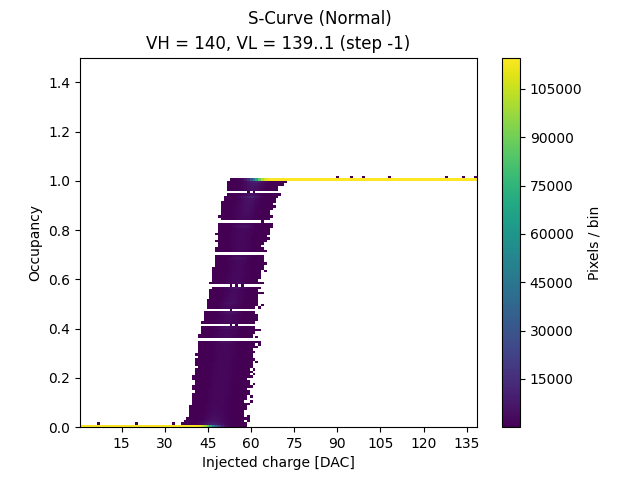
\includegraphics[scale=.6]{all_norm_thscan_140}
\caption{S-curves di tutti i pixel del flavor Normal della matrice con un impulso di iniezione di 140 DAC.}
\label{norm_scurve_140}
\end{figure}

Utilizzando questi valori, nessun pixel di questo flavor è risultato rumoroso e dunque non è stato necessario utilizzare alcuna maschera.

Come spiegato nella sezione (....) sono state fittate le distribuzioni delle threshold ottenute in due misure separate con un impulso di iniezione rispettivamente di 140 DAC e 200 DAC, mostrate in figura (...).

\begin{figure}
\centering
\subfigure[VH = 140 DAC]
{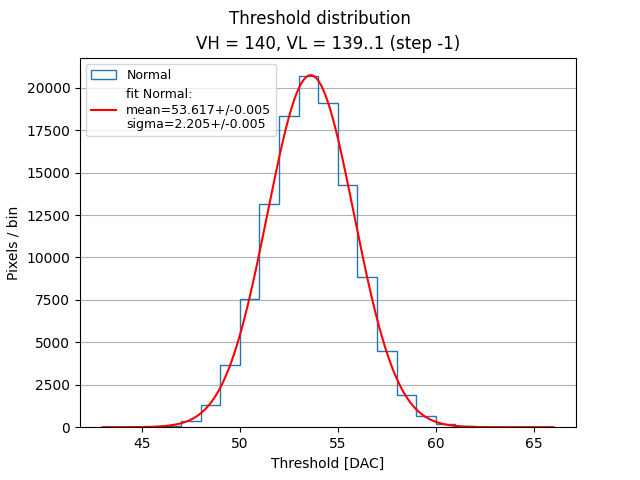
\includegraphics[scale=0.6]{all_norm_thdist_140}}\quad
\subfigure[VH = 200 DAC]
{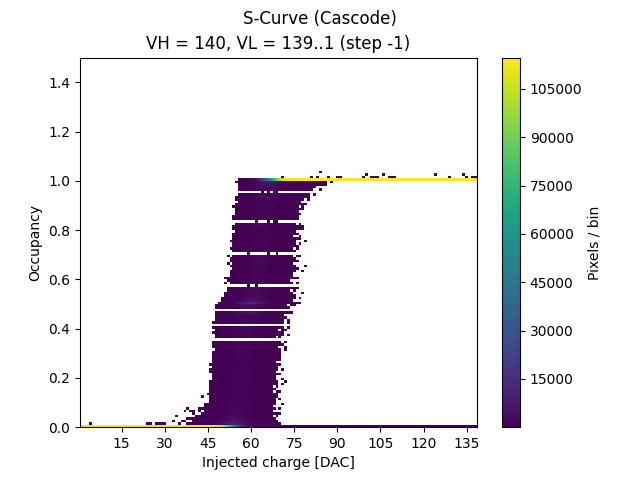
\includegraphics[scale=0.6{all_norm_thdist_200}}\\
\caption{Distribuzioni delle threshold prima della saturazione e alla saturazione massima.}
\label{thdist_norm}
\end{figure}

Per altezza dell'impulso di iniezione maggiore, in realtà sono state fatte 8 diverse misure, ciascuna su 28 colonne consecutive e tutte le righe. Sono stati poi messi insieme i dati per ricavare plot riassuntivi sull'intero flavor. Stessa cosa è stata fatta per il flavor \textbf{Cascode}.


\end{comment}

\subsubsection{Cascode FE}

\begin{comment}

Il secondo flavor \textbf{Cascode} comprende 512 righe (0-511) e 224 colonne (224-447) anch'esso per un totale di 114.688 pixel. Anche per queste misure sono stati utilizzati come valori dei registri quelli del TB@Desy riportati in tabella (riferimento) e anche qui non sono stati identificati pixel rumorosi.
In figura (...) le S-curves di tutti i pixel.

\begin{figure}
\centering
\includegraphics[scale=.6]{all_casc_thscan_140}
\caption{S-curves di tutti i pixel del flavor Cascode della matrice con un impulso di iniezione di 140 DAC.}
\label{casc_scurve_140}
\end{figure}

Anche qui sono state fittate le distribuzioni delle threshold, riportate in figura (...).


\begin{figure}
\centering
\subfigure[VH = 140 DAC]
{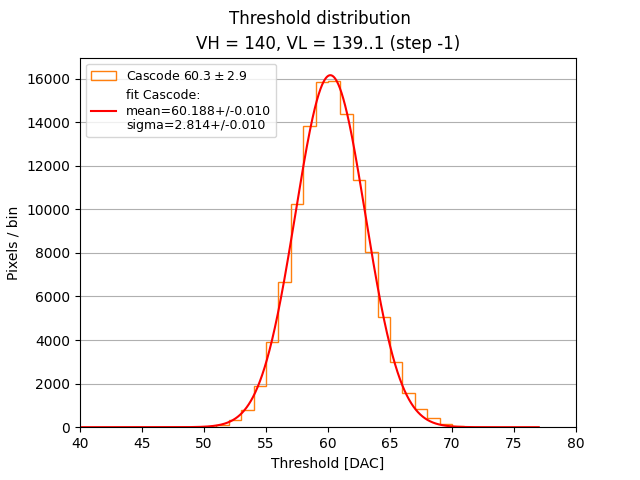
\includegraphics[scale=0.6]{all_casc_thdist_140}}\quad
\subfigure[VH = 200 DAC]
{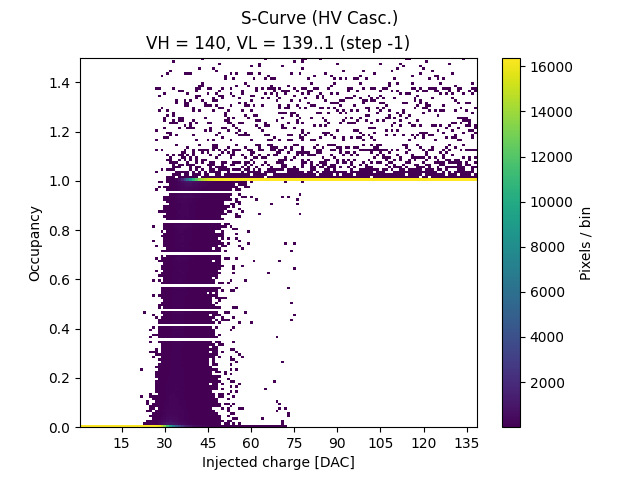
\includegraphics[scale=0.6{all_casc_thdist_200}}\\
\caption{Distribuzioni delle threshold prima della saturazione e alla saturazione massima.}
\label{thdist_casc}
\end{figure}

\end{comment}


\subsubsection{HV-Cascode FE}

\begin{comment}

Il terzo flavor \textbf{HV-Cascode} comprende 512 righe (0-511) per 32 colonne (448 -479) per un totale di 16384 pixel. Anche per questi ultimi due flavor HV, sono stati settati particolari valori dei registri, il cui funzionamento è stato studiato durante il Test Beam a Desy. Sono riportati nella tabella(ref).

\begin{table}
\centering
\begin{tabular}{c|c}
Registri & Default Settings (''GOE'') \\
\hline
ITHR & 30 \\
\hline
IBIAS & 60 \\
\hline
VRESET & 100 \\
\hline
ICASN & 8 \\
\hline
VCASP & 40 \\
\hline
VCASC & 228 \\
\hline
IDB & 100 \\
\hline
ITUNE & 53 \\
\hline
VCLIP & 255 \\
\hline
ICOMP & 80 \\
\hline
IDEL & 88 \\
\hline
IRAM & 50 \\
\hline
\end{tabular}
\caption{Settings dei principali registri utilizzati per il chip W14R12, flavors HV's durante il Test Beam a Desy.}
\label{tb_hv_settings}
\end{table}

Come visibile dalle S-Curves su tutta la regione interessata, con questa scelta dei parametri vi erano molti pixel rumorosi, che in questa fase delle misure, non sono stati mascherati.

\begin{figure}
\centering
\includegraphics[scale=.6]{all_HVc_thscan_140}
\caption{S-curves di tutti i pixel del flavor HV Cascode della matrice con un impulso di iniezione di 140 DAC.}
\label{hvc_scurve_140}
\end{figure}


Di seguito in figura (ref), i fit delle distribuzioni delle threshold per i due diversi impulsi di iniezione.

\begin{figure}
\centering
\subfigure[VH = 140 DAC]
{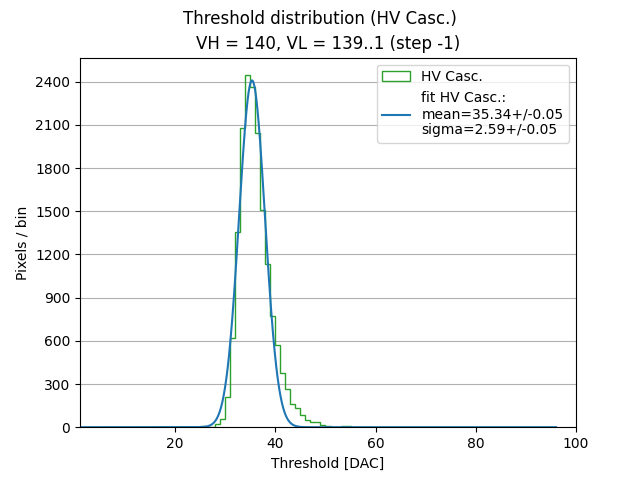
\includegraphics[scale=0.6]{all_HVc_thdist_140}}\quad
\subfigure[VH = 200 DAC]
{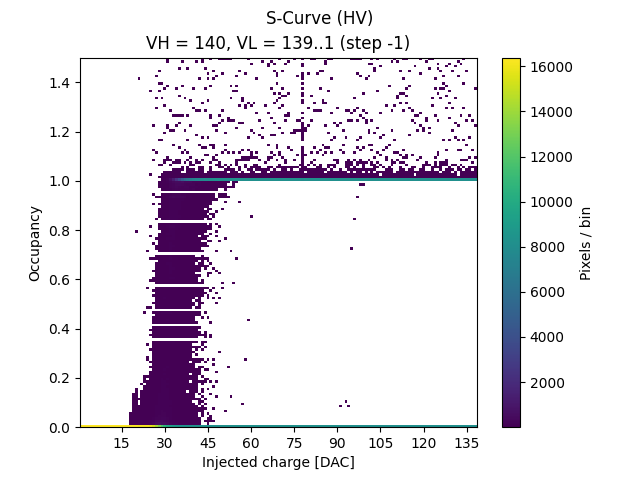
\includegraphics[scale=0.6{all_HVc_thdist_200}}\\
\caption{Distribuzioni delle threshold prima della saturazione e alla saturazione massima.}
\label{thdist_hvc}
\end{figure}


\end{comment}

\subsubsection{HV-Normal FE}

\begin{comment}
Il quarto ed ultimo flavor \textbf{HV-Normal} comprende 512 righe (0-511) per 32 colonne (448 -479) per un totale di 16384 pixel. Anche qui i registri sono stati settati ai valori riportati in tabella (ref). Di seguito in figura (ref), la S-curve su tutti i pixel e anche qui possiamo vedere diverso rumore a pixel noisy, non mascherati. In quest'ultimo flavor inoltre, le ultime 16 colonne non erano funzionanti, queste hanno restituito un picco di threshold a zero che è stato escluso dal plot della distribuzione delle threshold. Dunque in realtà in quest'ultimo pezzo della matrice, i pixel studiati sono stati la metà, ossia 8192.

\begin{figure}
\centering
\includegraphics[scale=.6]{all_HV_thscan_140}
\caption{S-curves di tutti i pixel del flavor HV Cascode della matrice con un impulso di iniezione di 140 DAC.}
\label{hv_scurve_140}
\end{figure}


Di seguito in figura (ref), i fit delle distribuzioni delle threshold per i due diversi impulsi di iniezione.

\begin{figure}
\centering
\subfigure[VH = 140 DAC]
{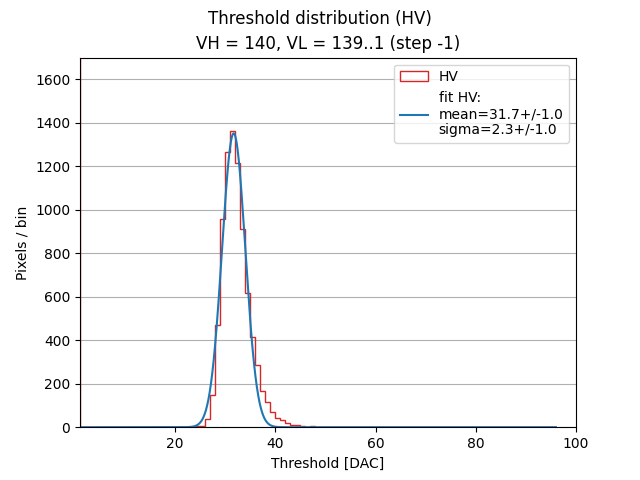
\includegraphics[scale=0.6]{all_HV_thdist_140}}\quad
\subfigure[VH = 200 DAC]
{\includegraphics[scale=0.6{all_HV_thdist_200}}\\
\caption{Distribuzioni delle threshold prima della saturazione e alla saturazione massima.}
\label{thdist_hvc}
\end{figure}



\end{comment}


\subsection{Noise and Equivalent Noise Charge (ENC)}
%\addcontentsline{toc}{subsection}{Noise and Equivalent Noise Charge (ENC)}

\subsection{Curve del Time Over Threshold (TOT) e fit}
%\addcontentsline{toc}{subsection}{Curve del Time Over Threshold (TOT) e fit}

\section{Caratterizzazione con le sorgenti radioattive}
%\addcontentsline{toc}{section}{Caratterizzazione con le sorgenti radioattive}

Fe55, Am241, Cd109, Sr190

\subsection{Calibrazione della capacità di iniezione}
%\addcontentsline{toc}{subsection}{Calibrazione della capacità di iniezione}


% --------------------------------------------
%		CONCLUSIONI 
%---------------------------------------------
\chapter{Conclusioni}
%\addcontentsline{toc}{chapter}{Conclusioni}




% --------------------------------------------
%		INDICE 
%---------------------------------------------
%\index{Conclusioni}
%\index{Pixel ibridi}
%\index{Ibridizzazione}
\printindex

% --------------------------------------------
%		BIBLIOGRAFIA 
%---------------------------------------------

% --------------------------------------------
%		ACRONIMI
%---------------------------------------------

% --------------------------------------------
%		LIST OF FIGURE AND TABLES 
%---------------------------------------------

\end{document}